\documentclass{minimal} % Classe básica para documentos simples.

\usepackage{lipsum}     % Gera texto de exemplo.
\usepackage{graphicx}   % Manipula imagens.
\usepackage{tikz}       % Cria gráficos e diagramas.
\usepackage{xcolor}     % Permite uso de cores.
\usepackage{qrcode}     % Gera códigos QR.
\usepackage{adjustbox}  % Redimensiona e alinha elementos.
\usepackage{multicol}   % Cria múltiplas colunas.
\usepackage{paracol}    % Colunas paralelas com mais controle.
\usepackage{wrapfig}    % Insere figuras com texto ao redor.
\usepackage{caption}    % Customiza legendas.
\usepackage{float}      % Controla posicionamento de figuras/tabelas.
\usepackage{fix-cm}     % Usa fontes escaláveis.
\usepackage[a4paper, left=0cm, right=1.5cm, top=0.5cm, bottom=0.5cm]{geometry} % Define tamanho do papel e margens.

% Define espaçamento entre colunas
\setlength{\columnsep}{0.5cm} 

% Definir as cores
\definecolor{primary}{HTML}{24249A}
\definecolor{secondary}{HTML}{6C93D2}

% Definindo os parâmetros
\newcommand{\dailyphrase}{\textit{``E conhecereis a verdade, e a verdade vos libertará.''} \\ João 8:32}
\newcommand{\chiefeditor}{Johannes Nogueira}
\newcommand{\websiteurl}{https://www.jornalsocrates.com.br}
\newcommand{\edition}{Ano \#1 | Nº \#123}
\newcommand{\startedattext}{Desde agosto de 2024}
\newcommand{\todaystr}{|Quinta-feira, 28 de novembro de 1991|}
\newcommand{\price}{R\$ 1,99}

\newcommand{\h}[1]{{\bfseries\fontsize{22}{24}\selectfont #1}}
\newcommand{\hh}[1]{{\bfseries\fontsize{16}{18}\selectfont #1}}

% Parâmetros:
% 1. Número da página
% 2. Título da seção
% 3. Data por extenso
\newcommand{\pageheader}[3]{
    \begin{tikzpicture}[remember picture, overlay]
        \node[anchor=east, text=primary, xshift=-0.5cm, yshift=-0.9cm] at (current page.north east) {#1};
        \draw[thick] ([xshift=-1.3cm, yshift=-0.7cm]current page.north east) -- ([xshift=-1.3cm, yshift=-1.1cm]current page.north east);
        \node[anchor=east, text=primary, xshift=-1.5cm, yshift=-0.9cm] at (current page.north east) {#2};
        \node[anchor=west, xshift=0.5cm, yshift=-0.9cm] at (current page.north west) {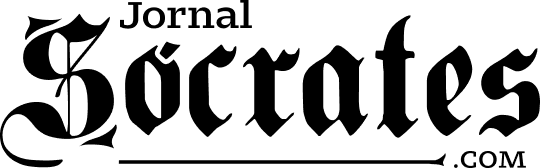
\includegraphics[height=0.6cm]{images/logo_black.png}};
        \draw[thick] ([xshift=3cm, yshift=-0.7cm]current page.north west) -- ([xshift=3cm, yshift=-1.1cm]current page.north west);
        \node[anchor=west, text=black, xshift=3.2cm, yshift=-0.9cm] at (current page.north west) {#3};
        \filldraw[fill=black, draw=none] 
        ([xshift=0.5cm, yshift=-1.4cm]current page.north west) rectangle ([xshift=-0.5cm, yshift=-1.5cm]current page.north east);
        \filldraw[fill=primary, draw=none] 
        ([xshift=0.5cm, yshift=-1.6cm]current page.north west) rectangle ([xshift=-0.5cm, yshift=-1.8cm]current page.north east);
    \end{tikzpicture}
}

\newcommand{\newsone}[3]{
    \begin{tikzpicture}[remember picture, overlay]
    
        \node[anchor=north west, xshift=0.5cm, yshift=-3cm] at (current page.north west) {\includegraphics[width=0.75\textwidth, height=0.75\textwidth]{#1}};    
        \node[anchor=north west, xshift=0.5cm, yshift=-2cm] at (current page.north west) 
        {\hh{#2}};
        \node[anchor=north east, xshift=-0.5cm, yshift=-3cm] at (current page.north east)  
        {\parbox{0.23\textwidth}{#3}};
        \draw[thick] ([xshift=-0.5\textwidth, yshift=11.5cm]current page.south) -- ([xshift=0.5\textwidth, yshift=11.5cm]current page.south);
    \end{tikzpicture}
}


\newcommand{\newstwo}[3]{
    \begin{tikzpicture}[remember picture, overlay]
        \node[anchor=south west, xshift=0.5cm, yshift=10.5cm] at (current page.south west) {\parbox{0.5\textwidth}{{\hh{Você sabia?}}}};
        \node[anchor=south west, xshift=0.5cm, yshift=10cm] at (current page.south west)  {\parbox{0.25\textwidth}{\textcolor{primary}{ \rule{0.15\textwidth}{0.1cm}}}};
        \node[anchor=north west, xshift=0.5cm, yshift=10.5cm] at (current page.south west) {\parbox{0.48\textwidth}{\begin{multicols}{2}
            \includegraphics[width=0.23\textwidth, height=0.25\textwidth]{#1}
            #3
        \end{multicols}}};
    \end{tikzpicture}
}


\newcommand{\newsthree}[3]{
    \begin{tikzpicture}[remember picture, overlay]
        \node[anchor=south west, yshift=10.5cm] at (current page.south) {\parbox{0.5\textwidth}{{\hh{Você sabia?}}}};
        \node[anchor=south west, yshift=10cm] at (current page.south)  {\parbox{0.25\textwidth}{\textcolor{primary}{ \rule{0.15\textwidth}{0.1cm}}}};
        \node[anchor=north west, yshift=10.5cm] at (current page.south) {\parbox{0.5\textwidth}{\begin{multicols}{2}
            \includegraphics[width=0.23\textwidth, height=0.25\textwidth]{#1}
            #3
        \end{multicols}}};
    \end{tikzpicture}
}




\begin{document}
\thispagestyle{empty}
\pageheader{31}{INFANTIL}{Quinta-feira, 28 de novembro de 1991}

\newsone{images/infantil_1.png}{23 de agosto: Dia do Aviador Naval}{No dia 23 de agosto, celebramos o Dia do Aviador Naval! Você sabia que os aviadores navais são pessoas muito especiais? Eles pilotam aviões que decolam e pousam em navios enormes, chamados porta-aviões. Esses aviões ajudam a proteger o nosso país e a realizar missões importantes.

Os aviadores navais são como super-heróis do céu! Eles voam alto, enfrentam desafios e sempre estão prontos para ajudar. Para se tornar um aviador naval, é preciso estudar bastante e treinar muito. Eles aprendem a voar em diferentes condições e a trabalhar em equipe.

Neste dia, podemos lembrar de todos os aviadores que arriscam suas vidas para manter a segurança de todos nós. Que tal colorir a imagem de um avião naval? Use suas cores favoritas e imagine como seria voar nas nuvens! Vamos celebrar juntos o Dia do Aviador Naval e agradecer a esses valentes pilotos que fazem a diferença!}

\newstwo{images/infantil_2.png}{}{Você sabia que os polvos têm três corações? Isso mesmo! Esses incríveis animais marinhos possuem um coração principal que bombeia sangue para o corpo e dois corações menores que se dedicam a bombear sangue para as brânquias, onde ocorre a respiração. O sangue dos polvos é azul, e isso acontece porque ele contém uma proteína chamada hemocianina, que é mais eficiente em transportar oxigênio em águas frias e profundas. Quando um polvo nada, o coração que leva o sangue para o corpo para de bater, o que faz com que eles prefiram se mover lentamente pelo fundo do mar. Além disso, os polvos são mestres do disfarce! Eles podem mudar de cor e textura para se camuflar em seu ambiente, usando células especiais na pele chamadas cromatóforos. Essas habilidades incríveis ajudam os polvos a se protegerem de predadores e a se tornarem caçadores astutos. O mundo dos polvos é realmente fascinante!}

\newsthree{images/infantil_3.png}{}{Você sabia que os polvos têm três corações? Isso mesmo! Esses incríveis animais marinhos possuem um coração principal que bombeia sangue para o corpo e dois corações menores que se dedicam a bombear sangue para as brânquias, onde ocorre a respiração. O sangue dos polvos é azul, e isso acontece porque ele contém uma proteína chamada hemocianina, que é mais eficiente em transportar oxigênio em águas frias e profundas. Além disso, os polvos são mestres do disfarce! Eles podem mudar de cor e textura para se camuflar no ambiente, usando células especiais na pele chamadas cromatóforos. E se você acha que eles são apenas criaturas curiosas, saiba que os polvos também são muito inteligentes! Eles podem resolver problemas, abrir frascos e até usar ferramentas. Então, da próxima vez que você pensar em um polvo, lembre-se de que ele é muito mais do que um simples habitante do mar!}

\end{document}\n\n\n